\chapter*{Upload File dan membuat aplikasi}
\section*{Upload file csv ke oracle dan merelasikan tabel lalu membuat aplikasi}
Langkah selanjutnya ialah load file csv. sehingga kita memiliki data tabel.Nanti tabel yang kita sudah upload akan kita gunakan dan relasikan di aplikasi. data file tersebut harus dalam excel dengan format csv. kita memiliki 5 data tabel. dan kita harus meload semua data itu. dengan meload data itu, maka data di excel akan masuk kedalam oracle express, beserta semua kolom yang ingin kita gunakan.
\section{Cara upload file csv}
berikut adalah cara untuk meload file ke oracle express.

\begin{enumerate}

\item[1] Upload file yang suda dibuat di excel dalam CSV. dalam kasus ini saya menggunakan file berikut
   


\item[2] Setelah itu lakukan import file excel ke apex, klik dropdown pada bagian ”SQL workshop”
lalu ”utilities” pilih ”Data Workshop”.

\begin{figure}
\item[3]lalu klik ”Load Data”, lalu pilih file excel yang akan di import, contoh disini
saya import file ”tabel dosen”. beri nama dan klik configure
    \begin{center}
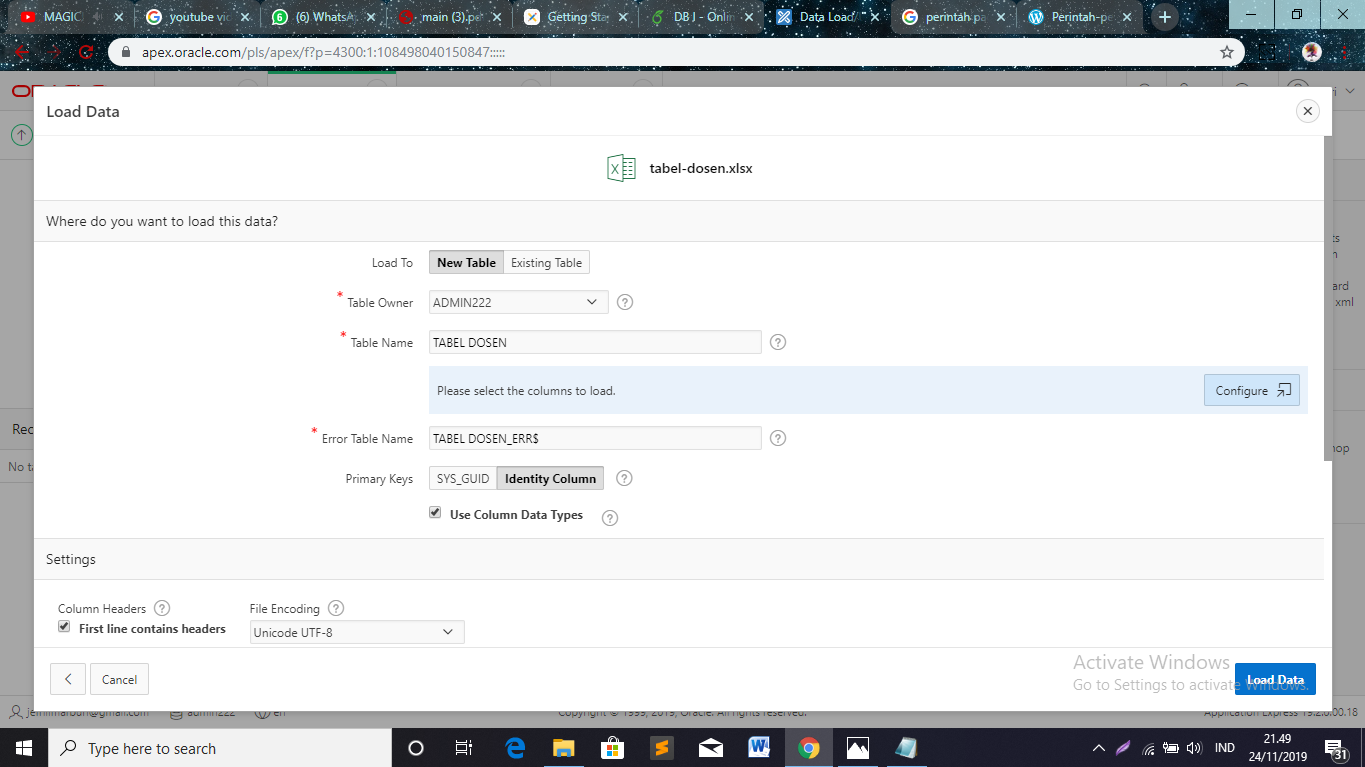
\includegraphics[scale=0.4]{apex/ss11.png}
    \caption{\textit{Load Tabel}}
        \end{center}

\end{figure}

\begin{figure}
\item[4]karna kita memerlukan semua kolom maka centang semua lalu save changes.
    \begin{center}
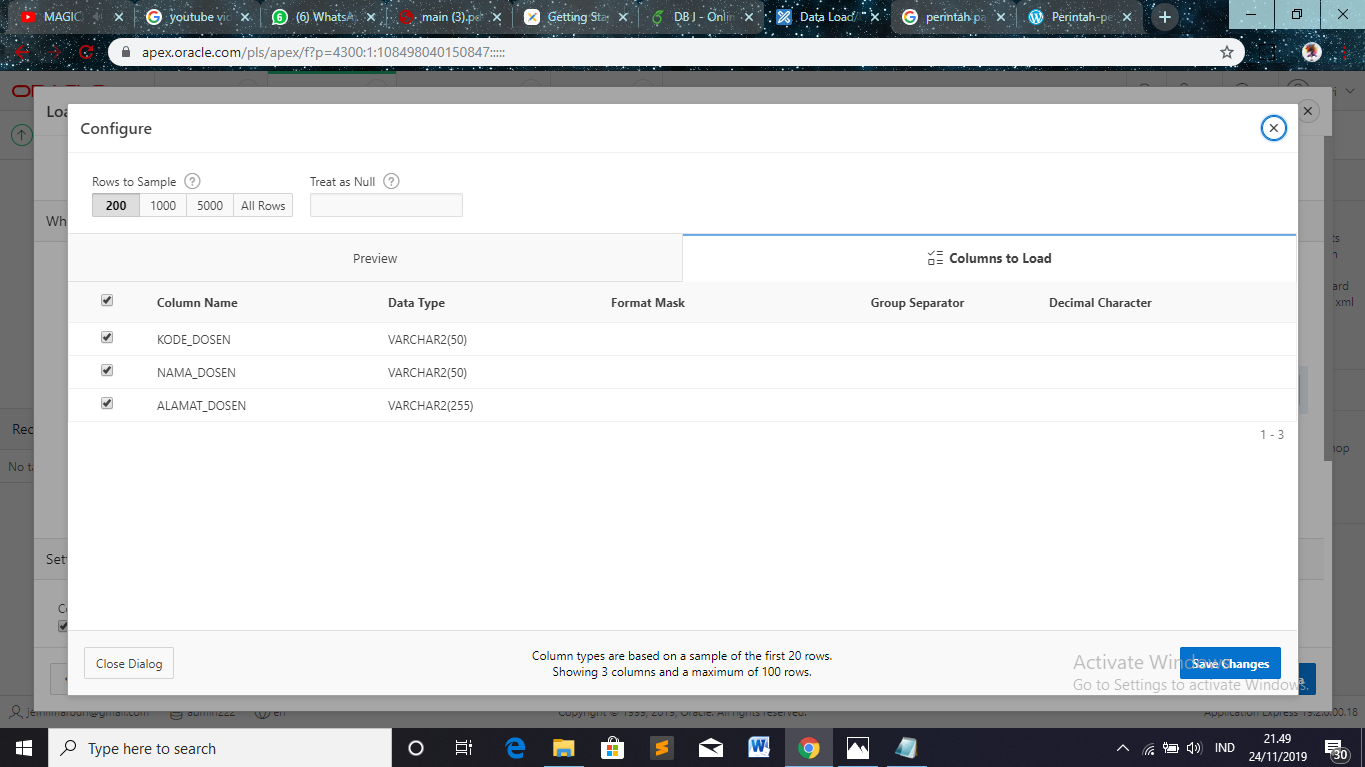
\includegraphics[scale=0.4]{apex/ss10.png}
    \caption{\textit{Configure Tabel}}
        \end{center}
\label{gambar}
\end{figure}

\begin{figure}
\item[5]lalu tabel telah berhasil di load.
    \begin{center}
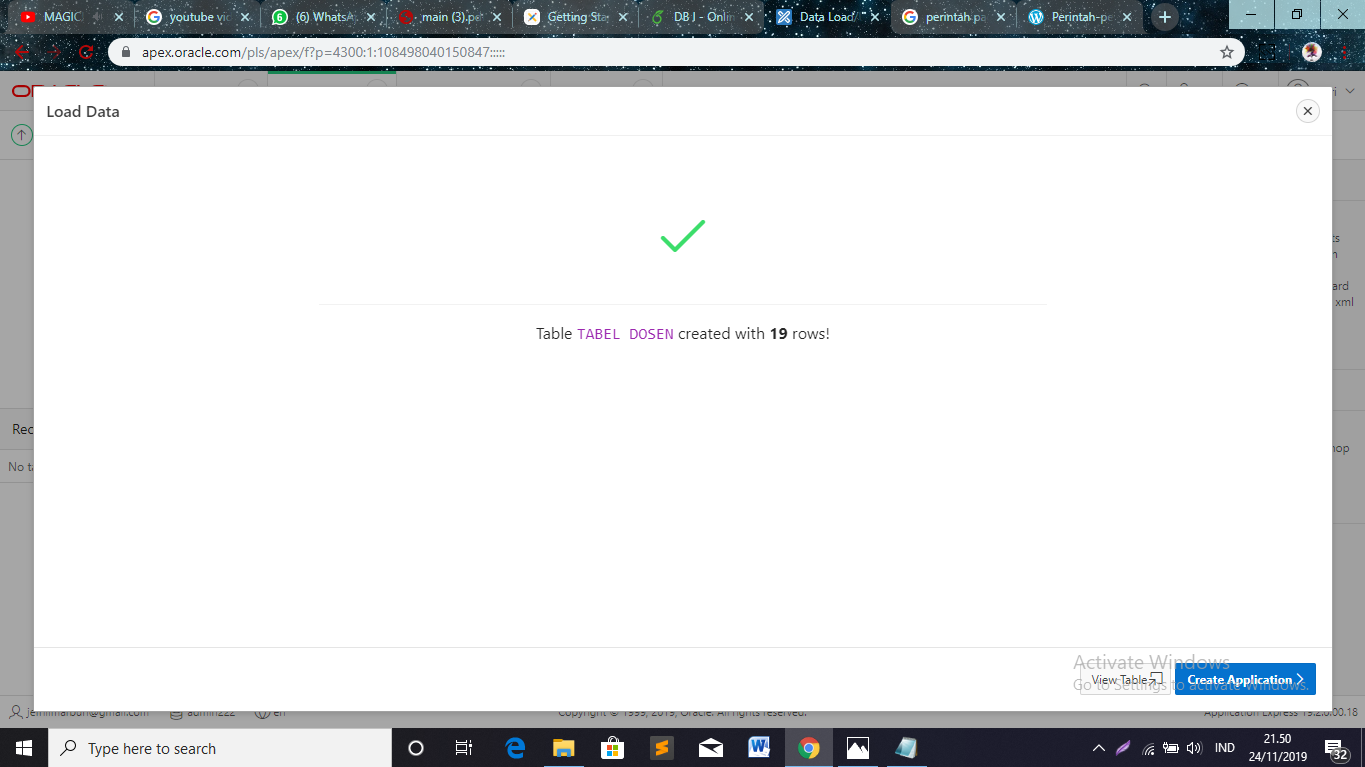
\includegraphics[scale=0.4]{apex/ss12.png}
    \caption{\textit{Tabel Berhasil diload}}
        \end{center}
\label{gambar}
\end{figure}

\begin{figure}
\item[6]lakukan kembali ke semua tabel yang ingin di load data.
\end{figure}

\begin{figure}
\item[7]Sekarang kita akan merelasikan tabel berikut
\end{figure}

\begin{figure}
\item[8]kita harus menghapus primary key default
\end{figure}

\begin{figure}
\item[9]Klik Data Workshop dan cari tabel yang akan kita hapus primary key nya,
disini saya akan menghapus primary key pada tabel mahasiswa, tabel dosen, tabel
mata kuliah, tabel jadwal, dan tabel nilai. Perintah yang di klik untuk menghapus
primary key adalah ”Drop Column”, lalu isikan column yang akan kita hapus
pada form ”Remove column” lalu klik next dan finish
    \begin{center}
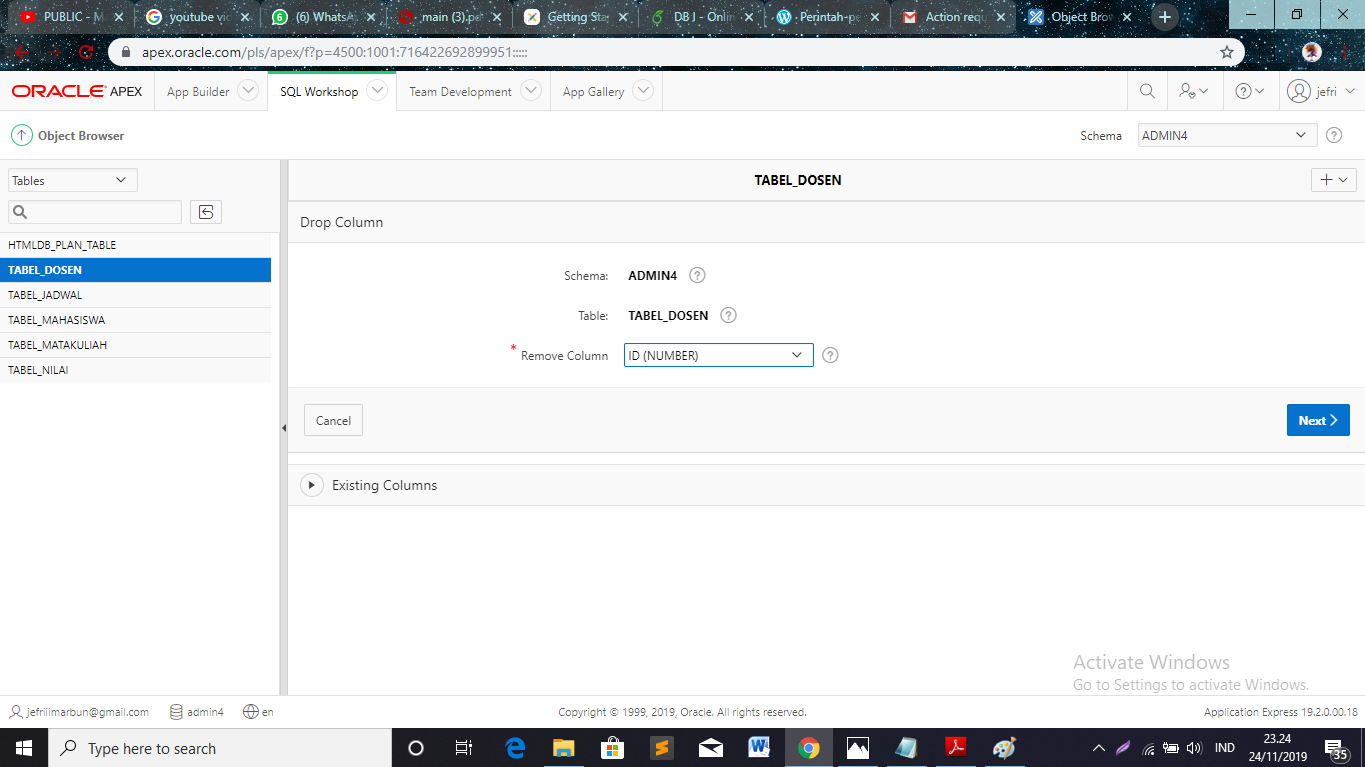
\includegraphics[scale=0.4]{apex/ss15.png}
    \caption{\textit{Tampilan SQL COMMANDS}}
        \end{center}
\label{gambar}
\end{figure}


\begin{figure}
\item[10]setelah itu kita melakukan pembuatan primary key, primary key harus unik. seperti berikut
    \begin{center}
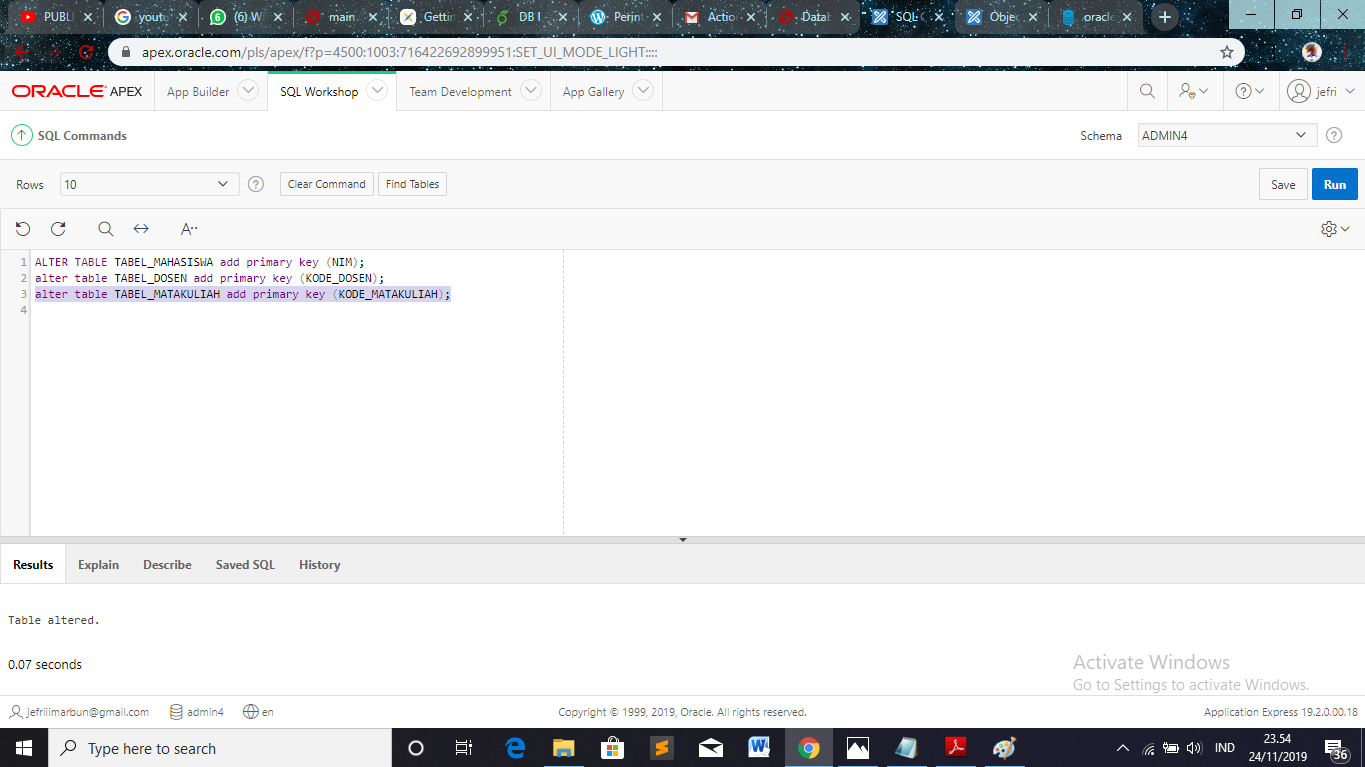
\includegraphics[scale=0.4]{apex/ss16.png}
    \caption{\textit{}}
        \end{center}
\label{gambar}
\end{figure}
\begin{figure}

\item[11]setelah itu kita melakukan pembuatan foreign key untuk bisa direlasikan
    \begin{center}
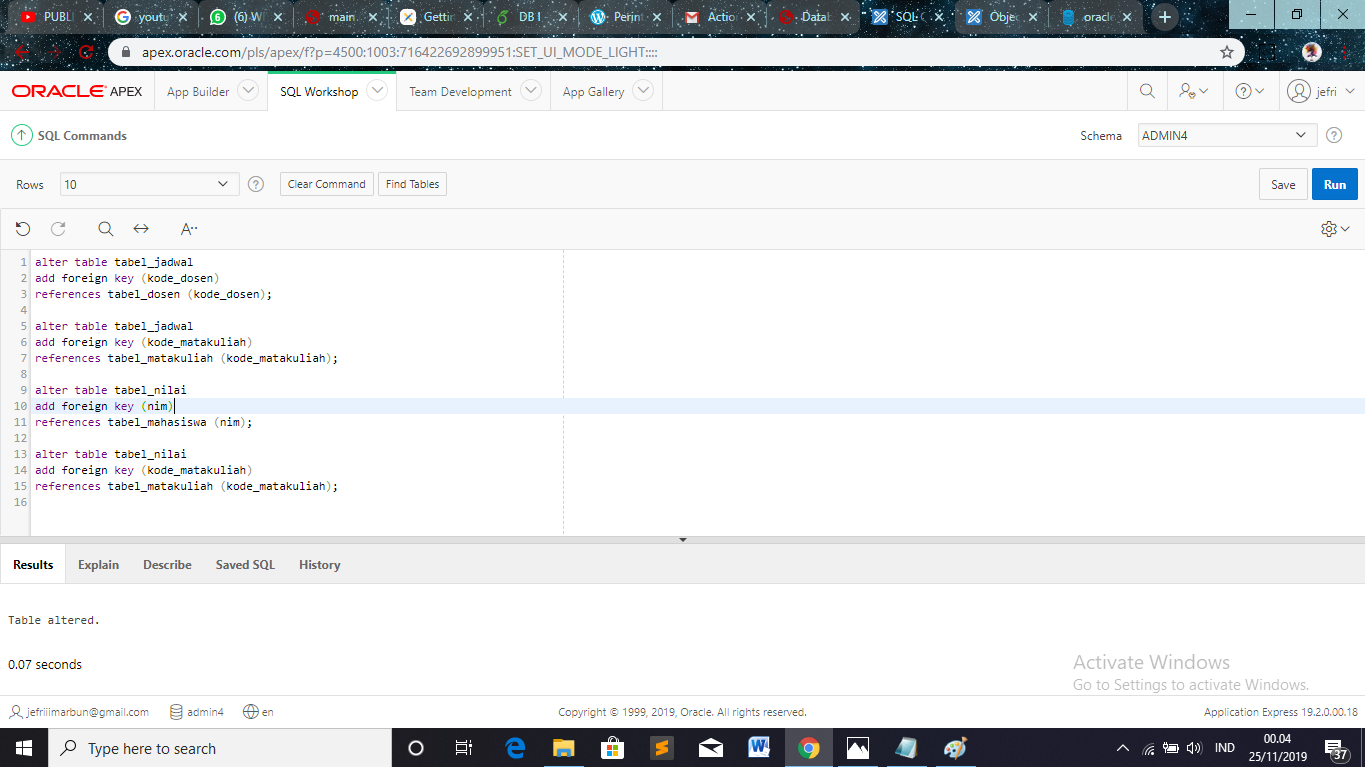
\includegraphics[scale=0.4]{apex/ss17.png}
    \caption{\textit{}}
        \end{center}
\label{gambar}
\end{figure}


\begin{figure}
\item[12]data sudah siap, setelah itu kembali ke halaman utama,ke app builder lalu pilih create
 \begin{center}
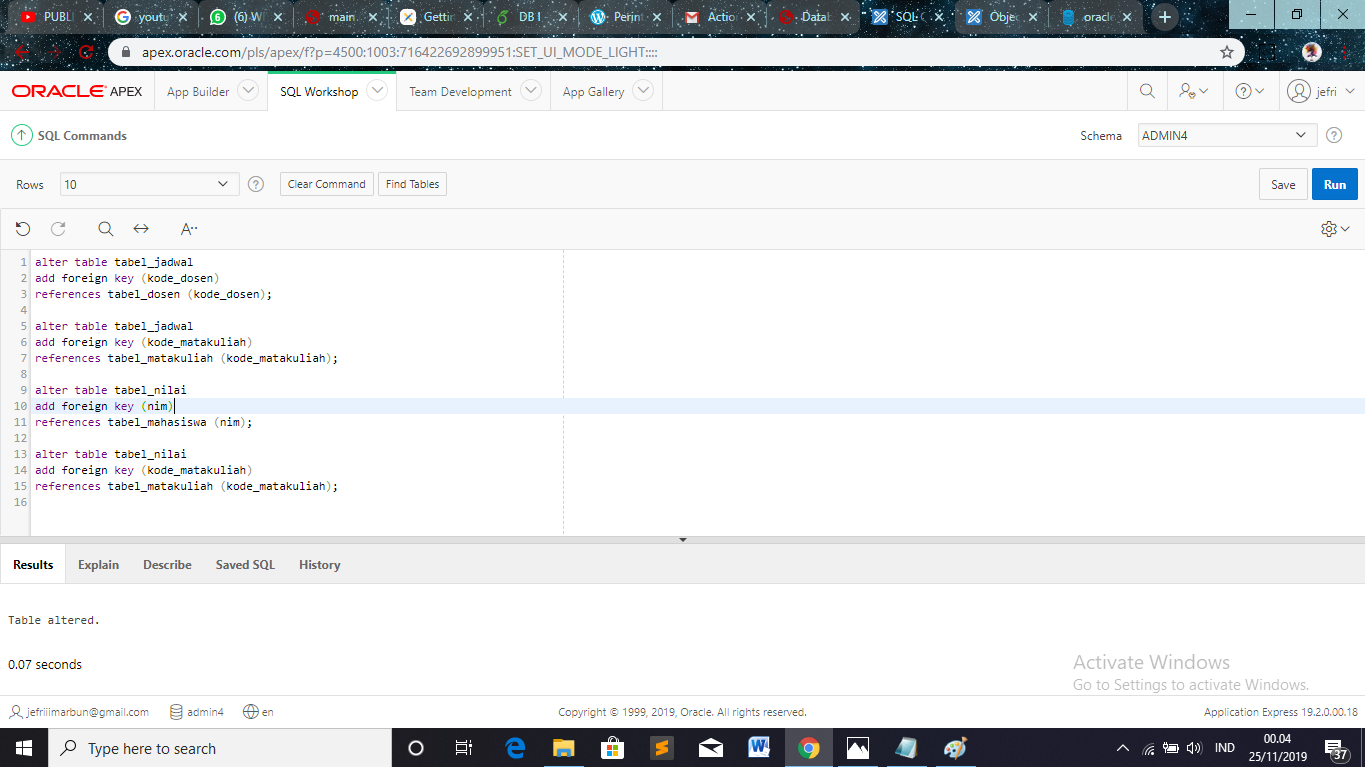
\includegraphics[scale=0.4]{apex/ss17.png}
    \caption{\textit{}}
        \end{center}
\label{gambar}
\end{figure}

\begin{figure}
\item[13]setelah itu pilih new application
 \begin{center}
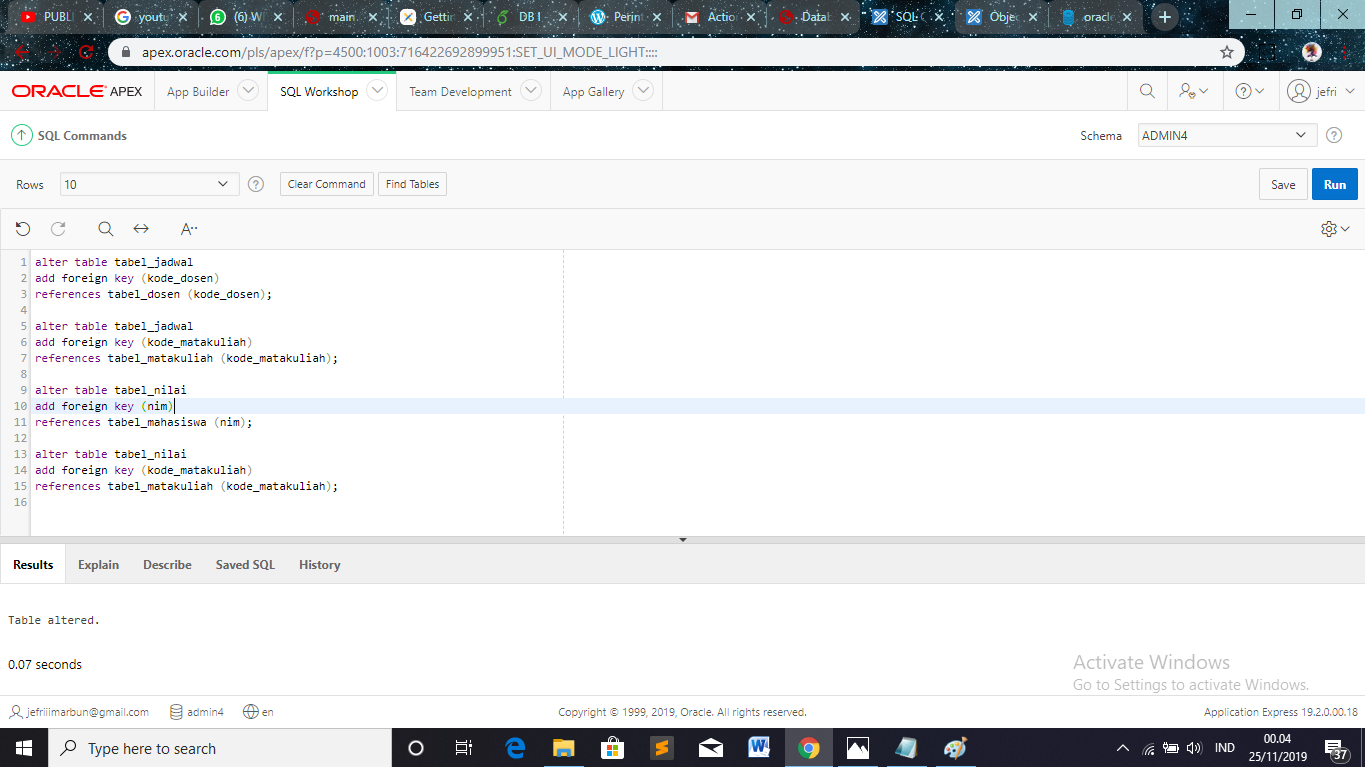
\includegraphics[scale=0.4]{apex/ss17.png}
    \caption{\textit{}}
        \end{center}
\label{gambar}
\end{figure}

\begin{figure}
\item[13]data sudah siap, setelah itu kembali ke halaman utama,ke app builder lalu pilih create lalu isi name
 \begin{center}
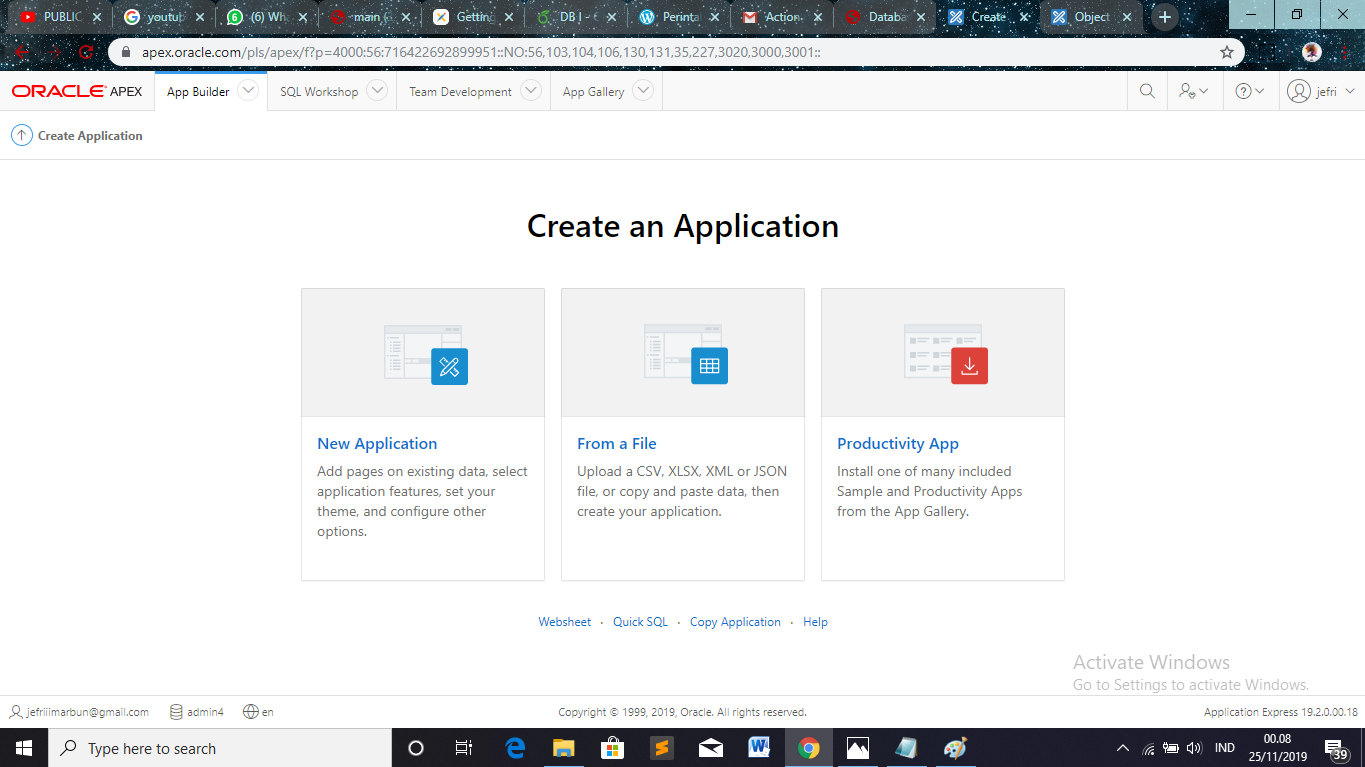
\includegraphics[scale=0.4]{apex/ss19.png}
    \caption{\textit{}}
        \end{center}
\label{gambar}

\end{figure}

\begin{figure}
\item[14]setelah itu pilih add page lalu pilih interactive report
 \begin{center}
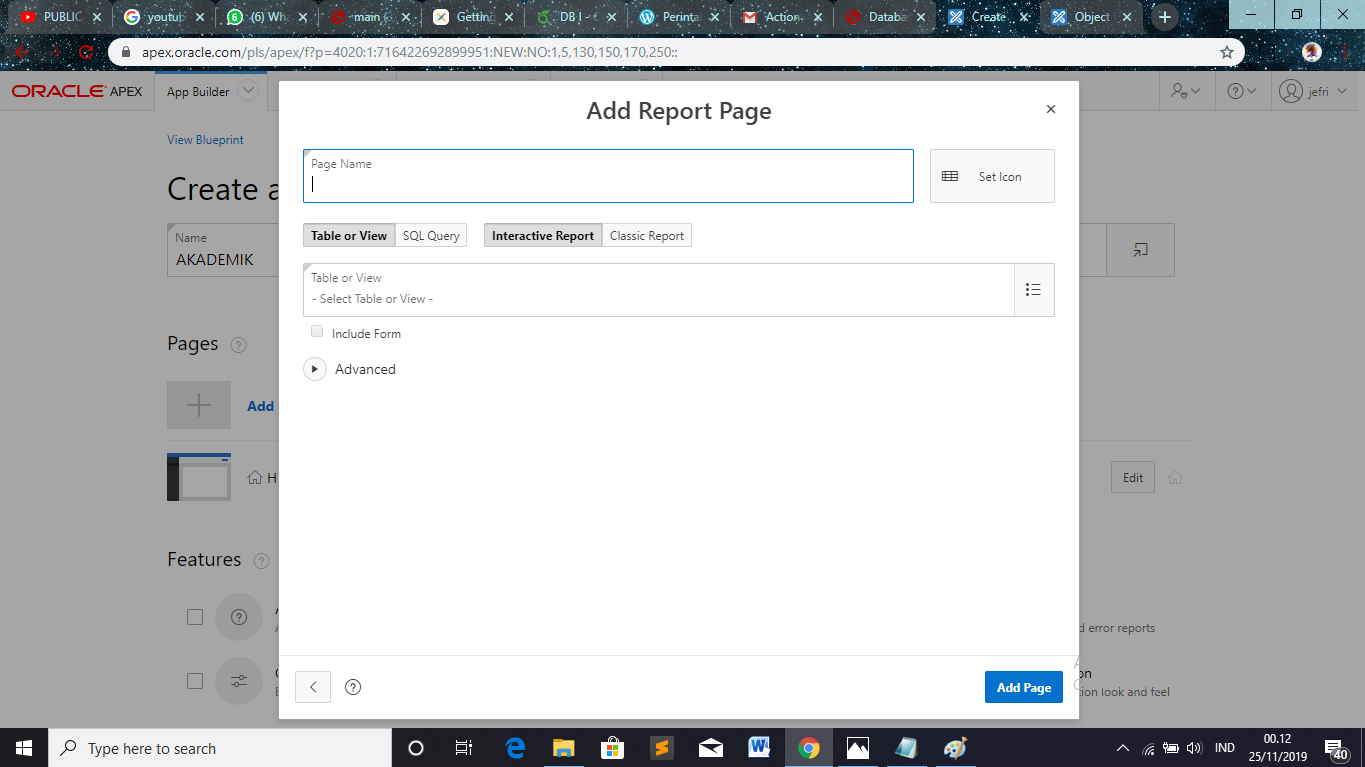
\includegraphics[scale=0.4]{apex/ss20.png}
    \caption{\textit{}}
        \end{center}
\label{gambar}
\end{figure}

\begin{figure}
\item[15]setelah itu add tabel mahasiswa, dosen, dan matakuliah secara bergantian jangan lupa add page terlebih dahulu sebelum pindah ke tabel selanjutnya
 \begin{center}
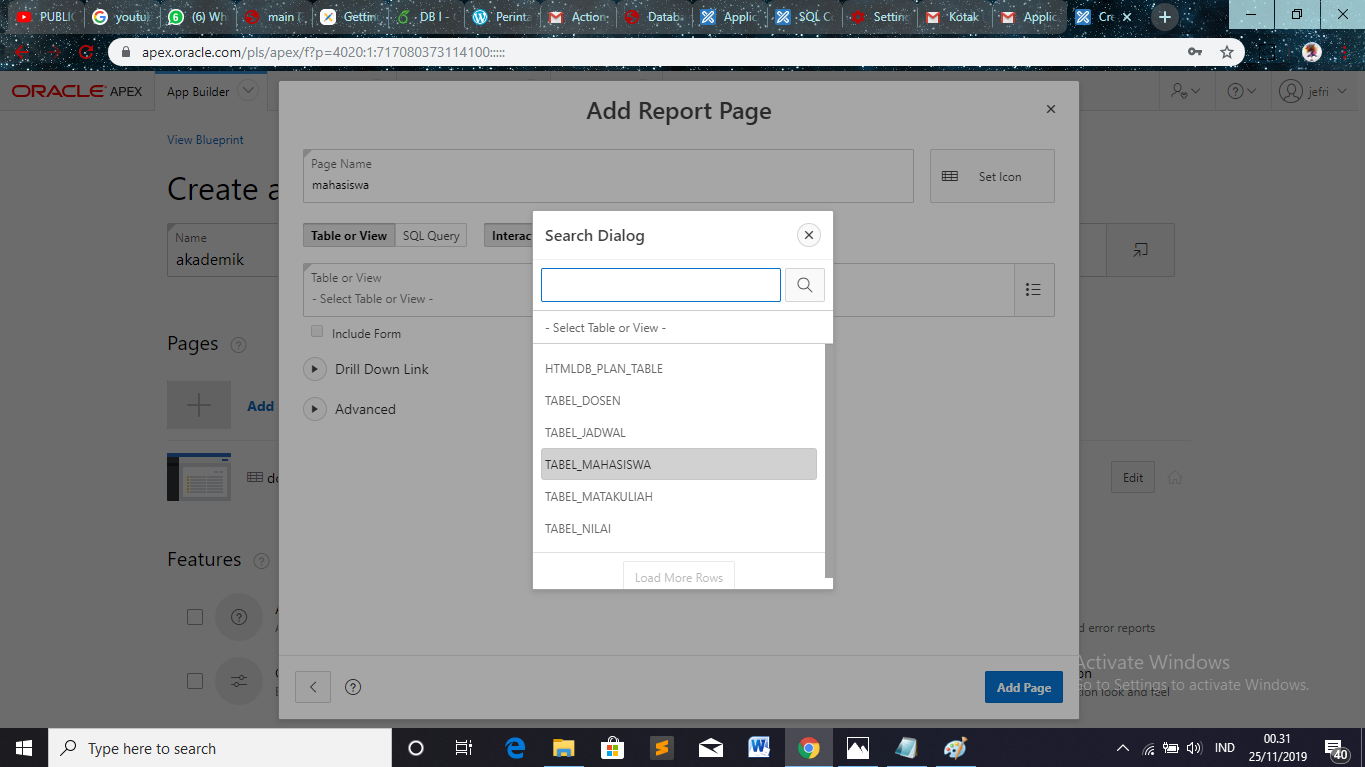
\includegraphics[scale=0.4]{apex/ss21.png}
    \caption{\textit{}}
        \end{center}
\label{gambar}
\end{figure}

\begin{figure}
\item[16]setelah itu pilih add page lalu pilih jadwal lalu isi dengan query berikut
 \begin{center}
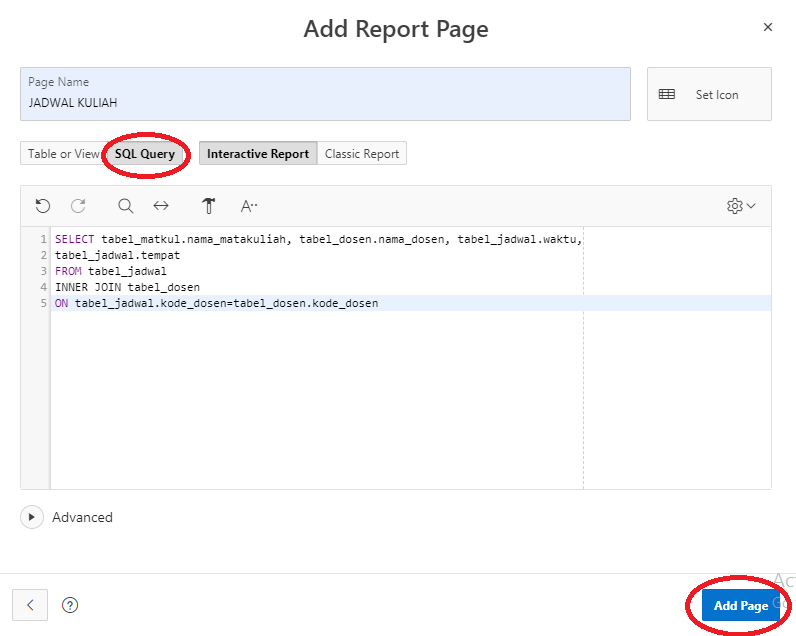
\includegraphics[scale=0.4]{apex/ss25.png}
    \caption{\textit{}}
        \end{center}
\label{gambar}
\end{figure}

\begin{figure}
\item[17]setelah itu pilih add page lalu pilih nilai lalu isi dengan query berikut
 \begin{center}
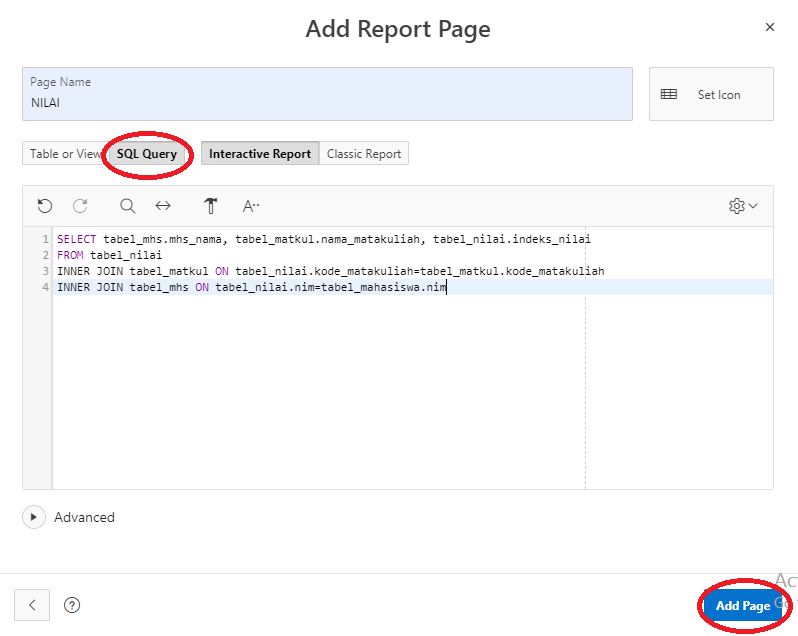
\includegraphics[scale=0.4]{apex/ss26.png}
    \caption{\textit{}}
        \end{center}
\label{gambar}
\end{figure}

\begin{figure}
\item[18]setelah itu pilih add page lalu pilih nilai lalu isi dengan query berikut
 \begin{center}
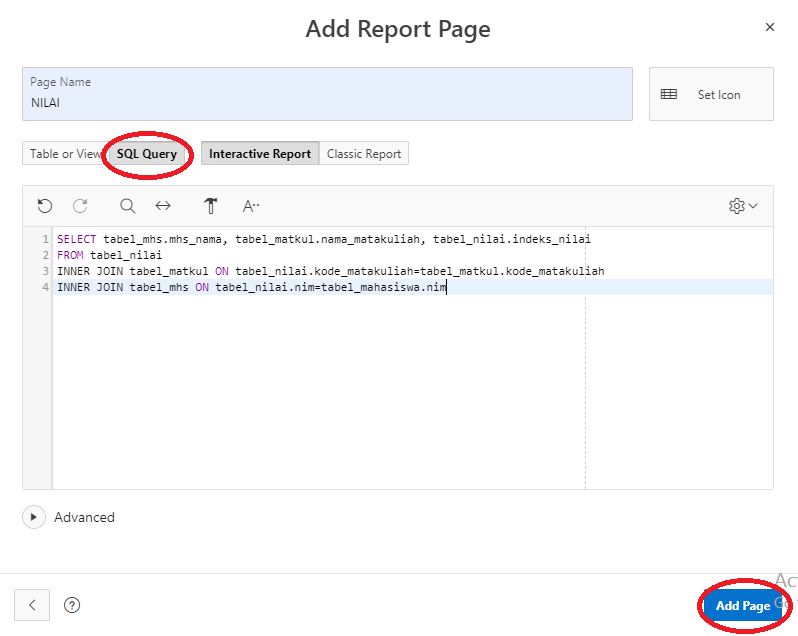
\includegraphics[scale=0.4]{apex/ss26.png}
    \caption{\textit{}}
        \end{center}
\label{gambar}
\end{figure}

\begin{figure}
\item[19]setelah itu pilih create application
 \begin{center}
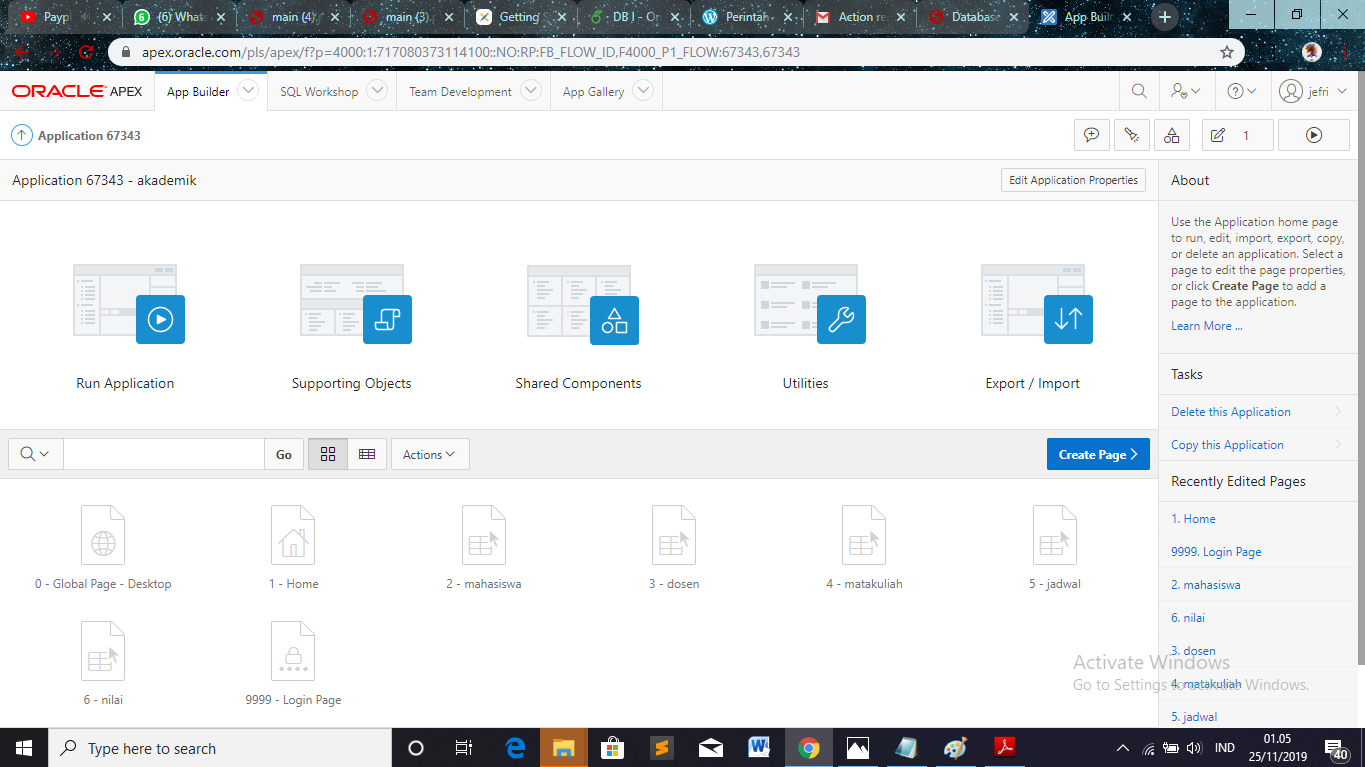
\includegraphics[scale=0.4]{apex/ss23.png}
    \caption{\textit{}}
        \end{center}
\label{gambar}
\end{figure}

\begin{figure}
\item[20]setelah itu run aplikasi maka anda harus login terlebih dahulu dan masuk ke aplikasi.
 \begin{center}
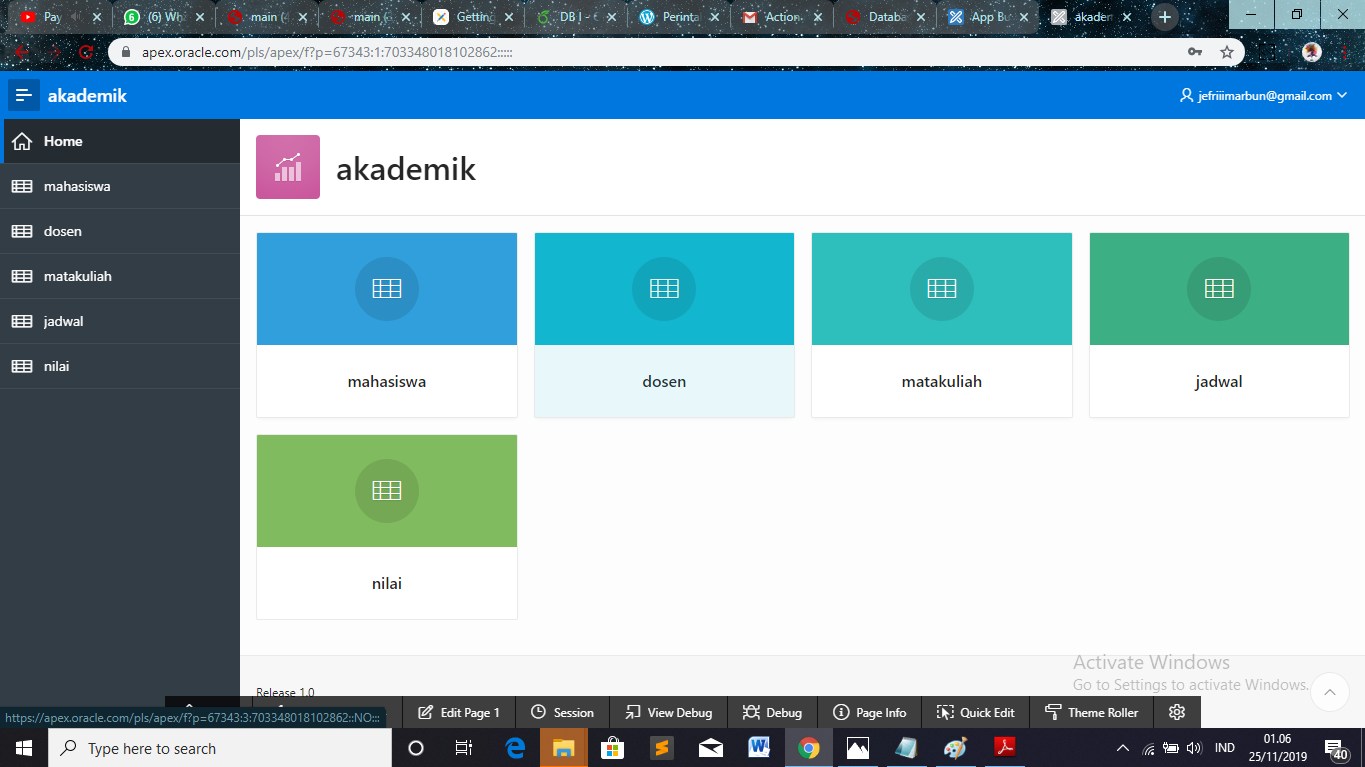
\includegraphics[scale=0.4]{apex/ss24.png}
    \caption{\textit{}}
        \end{center}
\label{gambar}
\end{figure}

\begin{figure}
\item[21]aplikasi sudah berjalan. terimakasih sudah membaca :)
\end{figure}





\end{enumerate}

